\section{Introduction}

\subsection{Surgery Robotics}

Surgery Robotics is a field of Surgery where the surgeon operaties on the patient via a computer, specialised equipment and robotic arms, 
to which the surgical tools needed for the operation are attached. According to surgical bibliography, robotics and laparoscopic procedures are used 
in general surgery, cardiothoracic surgeries, colon surgeries, gynecology, neurosurgery and orthopedics. \\

Robotic mechanisms were first introduced in Medicine, in 1987 with the first laparoscopic surgery of a cholecystectomy. Since then numerous laparoscopic 
operations have been performed and there has been a lot of improvements and innovations in this field. Such surgical operations are characterised as 
\textbf{minimally invasive}, because the surgical incisions made at the patient are very small and thus the probability of infection of the patient during 
or after the operation are very small, the hospitalization time is reduced (which means mean better and more efficient use of hospital resources) and the overall 
recovery of the patient is significantly faster and less painful. \\

However, traditional laparoscopic mechanisms have some downsides as well. First of all, the surgeon should operate in a mirrored-way, meaning that they should 
move at the opposite direction from what they saw at the screen (this effect is also known as the \textbf{fulcrum effect}), in order to reach the desired point of operation. Earlier laparoscopic tools had less 
degrees of freedom, which means less flexibility in motion control. Moreover these systems provided limited touch sensibility and feedback to the doctor they 
were very susceptible to the surgeon's micro movements and tremble. \\

The first application of robotics in Surgery appears in 1985, when Kwoh et al. \cite{Shao1985ANC} used a \textbf{PUMA 560}, a standard industrial robotic arm, to perform a neurosurgical biopsy, 
where the biopsy needle was inserted in the brain and guided with the help of Computed Tomography. This successful application was followed by the \textbf{PROBOT} surgical robot \cite{Probot1992}, 
which was developed at the Imperial College and used in a prostatectomy operation. Another example of an early surgery robot was the \textbf{ROBODOC} system \cite{Robodoc} developed by Integrated Surgical Supplies 
in Sacramento California, which was the first to be used in orthopedics for a hip replacement surgery and was also the first to be approved by the FDA (Food \& Drug Administration, organization responsible 
for medical devices, drugs etc.).

\begin{center}
\begin{figure}[H]
\centering
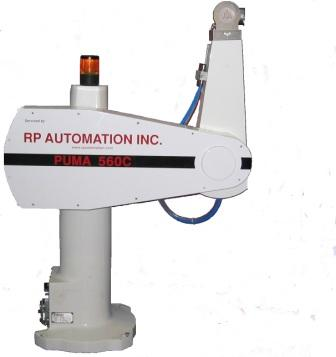
\includegraphics{images/Puma560.jpg}\\
\caption{The PUMA 560 robotic arm, which was the first to be used in surgery robotics in 1985}
\end{figure}
\end{center}

Some other important surgery robots are listed below:
\begin{itemize}
\item \textbf{AESOP® Endoscope Positioner}
\item \textbf{HERMES® Control Center}
\item \textbf{daVinci Surgical System®}
\item \textbf{SOCRATES Robotic Telecollaboration System}
\item \textbf{Raven-II} \cite{Raven2}: An open platform for collaborative research on surgical robotics.
\end{itemize}

\begin{center}
\begin{figure}[H]
\centering
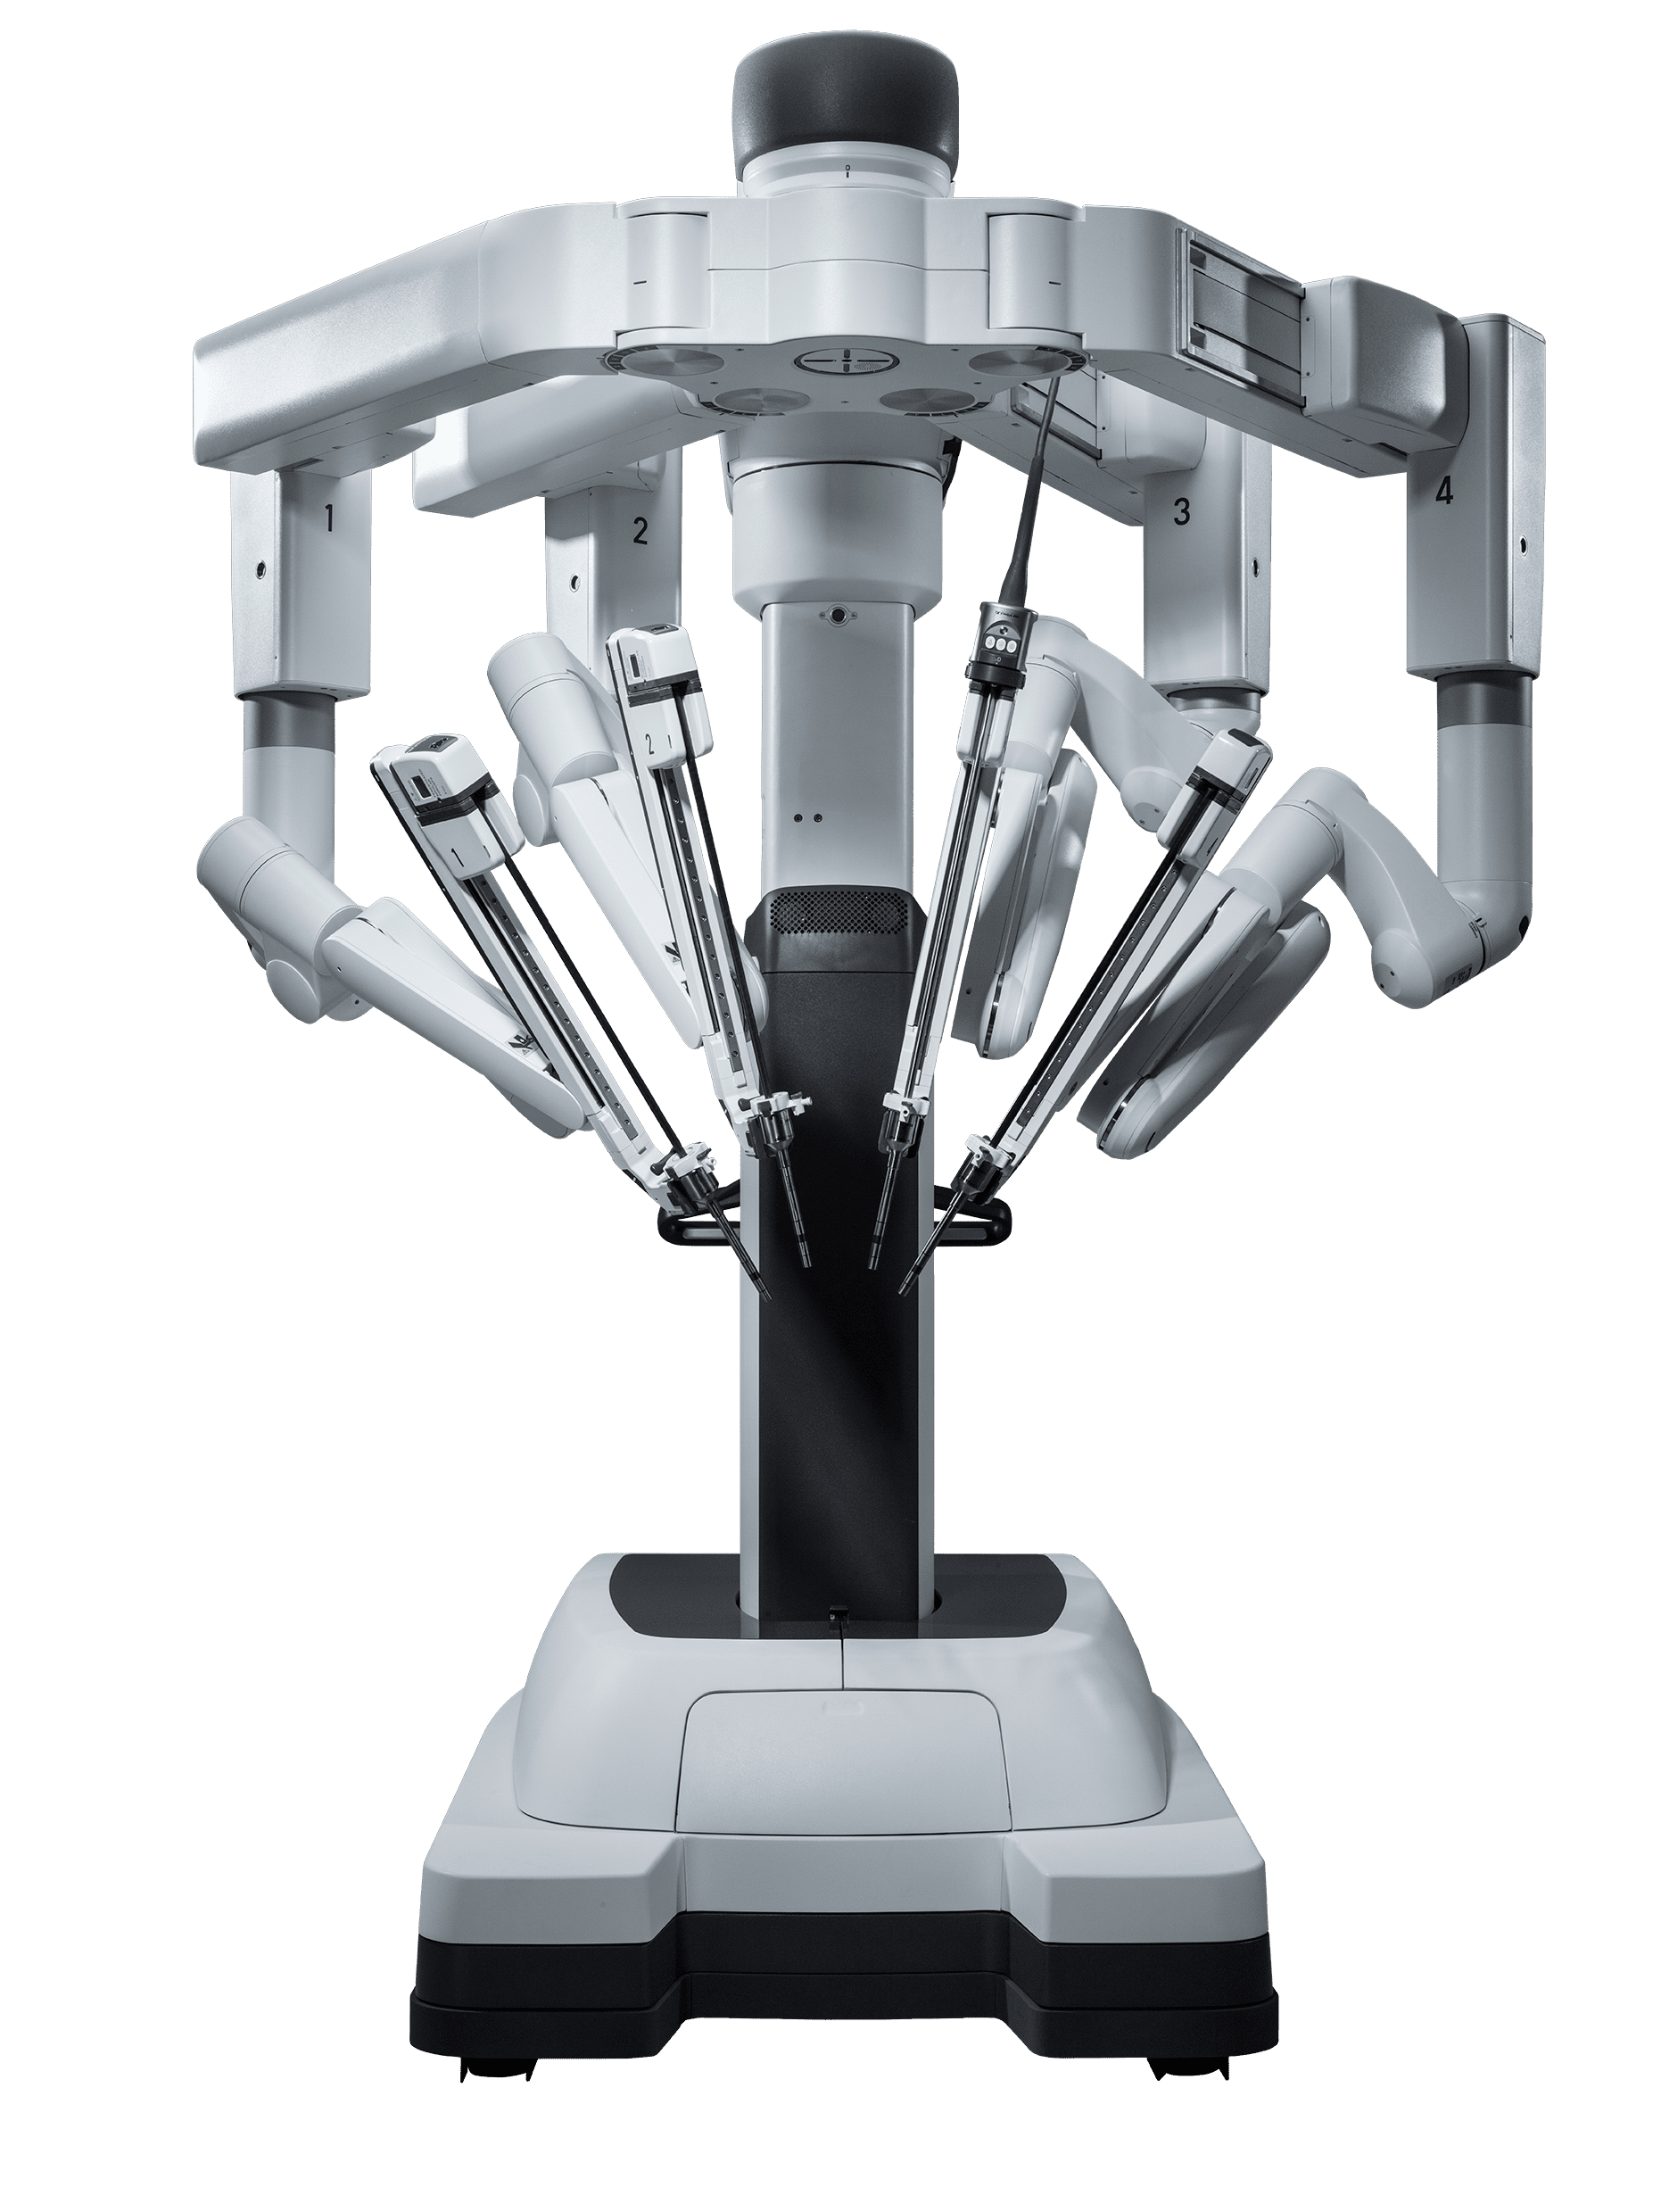
\includegraphics[width=8cm]{images/davinci-xi-patient-cart.png}\\
\caption{DaVinci Xi Patient Cart}
\end{figure}
\end{center}

\begin{center}
\begin{figure}[H]
\centering
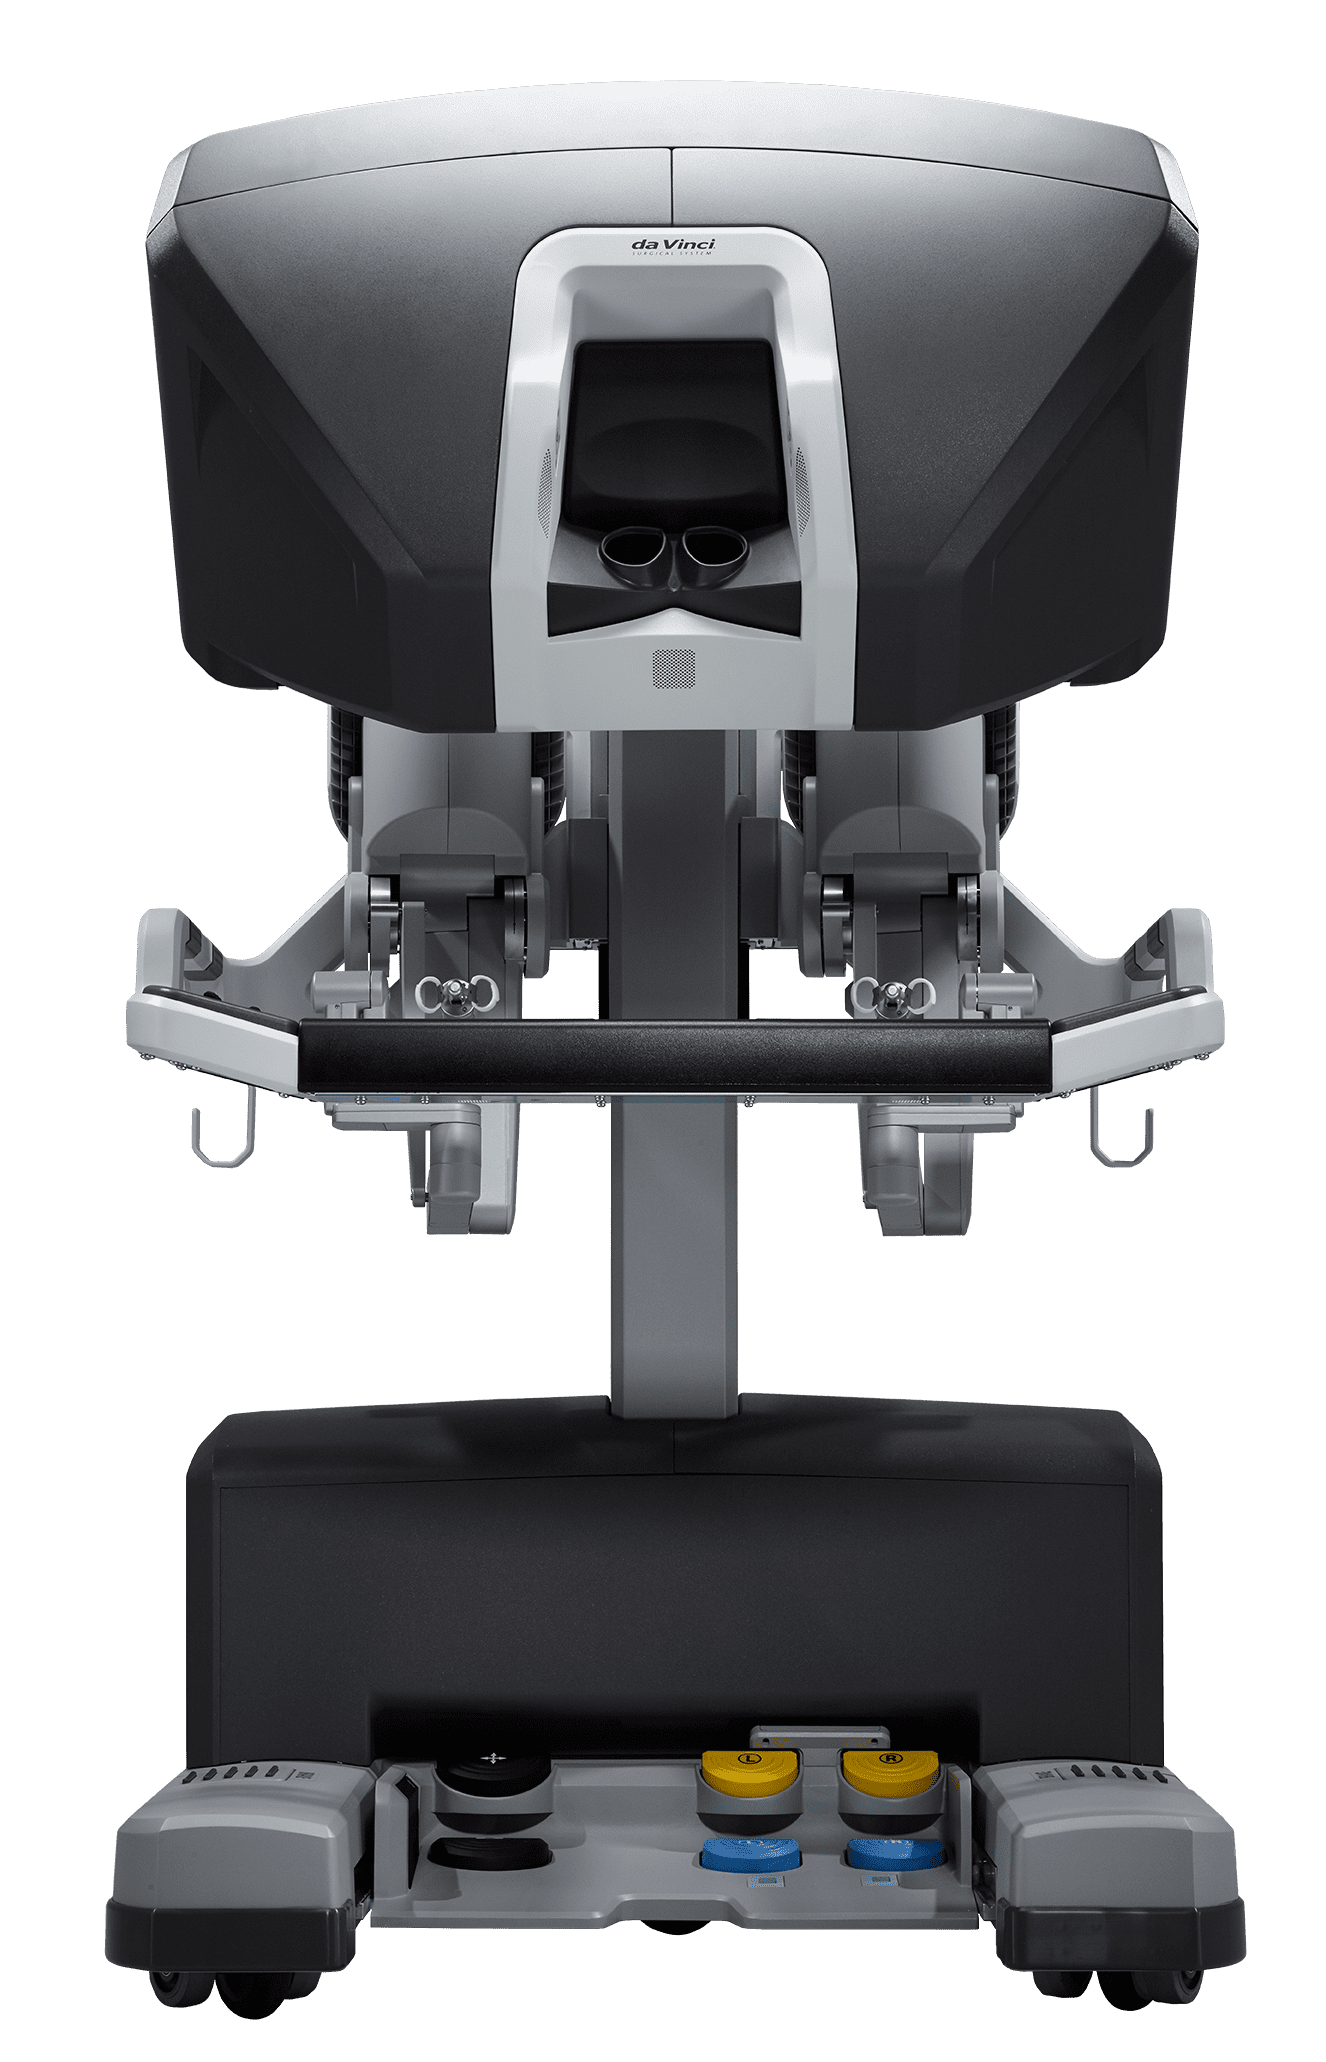
\includegraphics[width=8cm]{images/davinci-xi-surgeon-console.png}\\
\caption{DaVinci Xi Surgeon Console}
\end{figure}
\end{center}

\subsection{Bibliography Overview}

\subsection{Methodology \& Approach}